\section{Resultat}
% TODO

Projektets resultat är ett kodbibliotek för en haskelltolk. Här presenterar vi de olika modulerna som tolken består av. Koden finns att tillgå på GitHub: \url{http://github.com/johang88/haskellinjavascript}.

\subsection{Parser} 
Parserns uppgift är att ta användarens indata och konvertera den till en datastruktur 
som är lättare att hantera internt. Denna datastruktur kallas Abstract Syntax Tree (AST). 
Haskellstandarden har definerat upp en grammatik, ett antal regler, som definerar hur korrekt haskellkod ser ut och hur den ska tolkas.

Haskell är ett svårt språk att parsa då det inte är kontextfritt på grund av att kodens mening beror på blanksteg, 
Haskell tillåter även egendefinerade operatorer vilket också kan påverka kodens mening. 

För att parsa indatan använder vi ett bibliotek för att bygga parsers kallat JSParse \citep{jsparse}.
JSParse ger oss ett antal funktioner som vi använder för att definera grammatiken och konvetera den till vår interna struktur.

Som figur \ref{fig:parser_steg} visar, består parsern av tre mindre parsers, den första är en parser som hittar kommentarer och tar bort dessa. 
Det andra tar hand om kodens layout och gör om den till kontextfri kod. Den tredje gör om den kontextfria koden till vår AST.

\begin{figure}[H]
    \begin{center}
        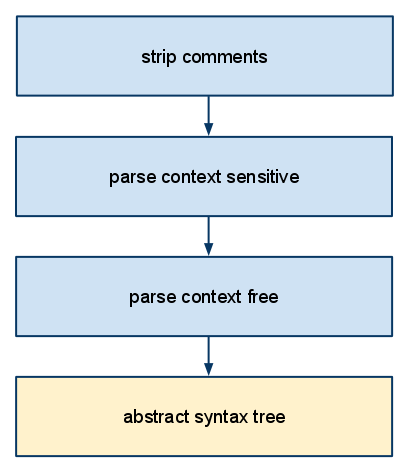
\includegraphics[width=.5\textwidth]{parser_1.png}
        \caption{Parserns olika steg}
        \label{fig:parser_steg} % Labels must come after caption!
    \end{center}
\end{figure}

Det var naturligt att dela upp parsern i tre olika steg. De tre olika stegen är skilda från varandra och vi kunde utveckla och testa dem individuellt.
Nedan följer ett exempel på parserns arbetssätt och de tre olika stegen:
\begin{lstlisting}
-- Kommentar
f x = case x of
    True -> False
    False -> True
\end{lstlisting}

Efter första steget:
\begin{lstlisting}
f x = case x of
    True -> False
    False -> True
\end{lstlisting}

Efter andra steget:
\begin{lstlisting}
f x = case x of {
    True -> False;
    False -> True
}
\end{lstlisting}

Efter det tredje steget är en AST genererad.
\begin{lstlisting}
Function("f", Lambda("x", 
    Case(VariableLookup("x"), [
        [PatternConstructor("True"), PatterConstructor("False")],
        [PatternConstructor("False"), PatterConstructor("True")],
    ])
))
\end{lstlisting}

\subsubsection{Steg 1 - Ta bort kommentarer}
Det första steget använder en parser som identifierar och tar bort kommentarer. 
Haskell har två olika kommentarsstiler, enkelradiga börjar med \emph{--} och slutar vid första radbytet och 
nästlade som kan gå över flera rader börjar med \emph{\{-} och slutar med \emph{-\}}.

\subsubsection{Steg 2 - Konvertera till kontextfri}
Det andra steget delar upp koden i dess ord och symboler samtidigt som den dekoreras med indenteringsnivåer enligt en algoritm % TODO vilken algoritm, k'a'lla
som är specifierad i haskellstandarden. Därefter användads en annan algoritm från standarden för att sätta in måsvingar och semikolon på rätt platser. % samma, vilken algoritm, TODO 
När de två algoritmerna är klara sätts koden ihop igen och skickas vidare till nästa steg.

En regel är att ett inre block inte får vara mindre indenterat än det omslutande blocket, exempelivs:
\begin{lstlisting}
case x of
    True -> ...
\end{lstlisting}
Här är \emph{True -> ...} ett inre block till \emph{case} och mer indenterat.

Ett annat exempel är:
\begin{lstlisting}
let x = 5
    y = 4
in x + y
\end{lstlisting}
Den korrekta översättningen är:
\begin{lstlisting}
let { x = 5; y = 4 } in x + y
\end{lstlisting}
För att översätta detta korrekt kommer parsern ihåg den aktuella nästlingsnivån av "let"-uttryck och var deras repsektive "in"-uttryck befinner sig. 
Den avslutande måsvingen sätts in där ett matchande "in"-uttryck påträffas.

Ett exempel som inte översätts korrekt:
\begin{lstlisting}
[x | let x = 2]
\end{lstlisting}
Den korrekta översättningen är:
\begin{lstlisting}
[x | let { x = 2 }]
\end{lstlisting}
Men det blir:
\begin{lstlisting}
[ x | let { x = 2 ] }
\end{lstlisting}
Anledningen är att endast nästlingen av \emph{let} och \emph{in} sparas, men här finns inget \emph{in}.
För att lösa felet måste parsern hålla reda på antalet paranteser, måsvingar, hakparanteser och komman efter ett let-uttryck och när en symbol som gör det ogiltligt 
med en avslutande måsvinge påträffas sätts måsvingen in precis innan symbolen.

\subsubsection{Steg 3 - Skapa AST}
Det tredje steget är en parser för den kontextfria varianten av Haskell som den är definerad i standarden. 
Samtidigt som koden tolkas byggs en AST upp. Parsern består av en liten parser för varje grammatisk regel som är definerad i haskellstandarden 
dessa parsers kombineras ihop för att bilda den slutgiltliga parsern. Det resulterar i ett träd av parsers, en parser för hela programmet som har flera mindre parsers under sig.

Exempel:
Definitionen i haskellstandarden:
\begin{lstlisting}
gdrhs -> gd = exp [gdrhs]
rhs -> exp [where decls]
     | gdrhs [where decls]
\end{lstlisting}
Dess respektive parsers:
\begin{lstlisting}
var gdrhs = gdrhs_action(
    repeat1(gdrhs_fix_list_action(sequence(ws(gd), 
                expectws('='), ws(exp)))));

var rhs = choice(
    decl_rhs_action(sequence(expect(ws('=')), ws(exp), 
         optional(sequence(expect(ws("where")), ws(decls))))),
     sequence(ws(gdrhs), optional(sequence(expect(ws("where")), 
         ws(decls))))
);
\end{lstlisting}

Här används \emph{choice} för att tolka de två olika alternativen i \emph{rhs} och om vi tittar närmare på \emph{gdrhs} 
så ser vi att det är en rekursiv funktionen vilket vi implementerar med \emph{repeat1} för att få en lista med minst en uppreprning.

Parsern använder den metod som är specifierad i Haskell 2010 \citep{haskell2010} för att lösa företrädesreglerna (precedence levels) för operatorer då denna metoden är enklare än den som är definerad i Haskell 98. 
Anledningen till att företrädesreglerna inte kan defineras direkt i parsern är att Haskell använder sig av användardefinerade företrädesregler.
Metoden fungerar så att den löser företrädesreglerna först efter ett uttryck har parsats till en lista med operatorer 
och uttryck, när en operator påträffas i listan slås dess företrädesnivå upp i en tabell och ett träd med 
operatorer och uttryck skapas. Sista används trädet för att generera en AST för uttrycken.

\subsubsection{JSParse}
Vi använder en modifierad version av JSParse där vi har korrigerat två fel och lagt till fler parsers. Felen vi korrigerade var i butnot-parsern och i choice-parserns cachefunktion. 
Choice-parsern cachade resultat från parsers som misslyckades och det cachade resultatet användes i senare parsers, 
vi löste det med en stackbaserad cache där cachen för en parser som misslyckas raderas.

Parsers som vi har lagt till:
\begin{enumerate}
    \item{\emph{repeatn}: en parser som upprepar en parser minst \emph{n} antal gånger}
    \item{\emph{expectws}: en parser som tillåter blanksteg och inte retunerar någon ast, är en kombination av JSParse inbyggda parsers \emph{expect} och \emph{whitespace}}
\end{enumerate}



\subsection{Interpretator}
Interpretatorns uppgift är att tolka det abstrakta syntaxträdet. Under interpreteringen används flera datastrukturer vars uppgift och struktur anges här.

\subsubsection{Thunk}
En Thunk är en avstannad beräkning, en continuation. En Thunk består av en Env och en Expression.

\begin{lstlisting}
data Thunk = Closure Env Expression
\end{lstlisting}

Haskell måste använda sig av non-strict evaluation vilket innebär att en uträkning inte får köras ifall den inte behövs. När en uträkning körs så innebär det att den resulterar i flertalet Thunks för de delar av beräkningen som ännu inte behövs. När värdet av en Thunk behövs kommer den att tvingas till en \emph{weak head normal form} (WHNF) eller en ny Thunk. Anledningen till detta är att vi på så sätt minskar användandet av rekursion vilket minskar risken att vi får ett runtime error.

\subsubsection{Weak Head Normal Form}
En WHNF är ett partiellt evaluerat uttryck. Uttrycket har blivit evaluerat så långt att vi är säkra på att det retunerar något typ av värde, alltså något som inte är undefined. Ofta innehåller en WHNF referenser till ännu icke evaluerade uttryck, om de inte gör det sägs uttrycket vara i Normal Form.

\begin{lstlisting}
data WeakHead 
    = Data Identifier [HeapPtr]
    | LambdaAbstraction Env Pattern Expression
    | DelayedApplication Env Int [Declaration] [HeapPtr]
    | Primitive
\end{lstlisting}

En Data är resultatet av att applicera en algebraisk datakonstruktor på dess argument. Argumenten ges som en lista av HeapPtr, det vill säga en lista av evaluerade eller icke evaluerade uttryck. Exemplevis resulterar Just 1 i en Data med Identifiern Just och en HeapPtr till det icke evaluerade uttrycket 1.

En LambdaAbstraction är körningsrepresentationen av en lambdafunktion, en Env är bunden till lambdafunktionen.

En DelayedApplication är ett specialfall av en LambdaAbstraction. Vi avsockrar inte Haskells funktionsdeklarationer vilket innebär att pattern matching sker även vid funktionsapplikation och inte bara i Case satser. Detta betyder att vi måste samla alla argument till en funktion innan vi kan avgöra vilket funktionsalternativ som skall användas. En vidare beskrivning finns i kapitlet Declaration.

En Primitiv är ett Javascript-värde, till exempel en integer eller en double.

\subsubsection{HeapPtr}
De flesta implementationer av Haskell använder sig av Lazy Evaluation, vilket innebär att en Thunk kommer att tvingas maximalt en gång. I vår implementation används HeapPtr som en wrapper runt en Thunk, när en HeapPtr dereferenceras kommer Thunk att tvingas till en WHNF och HeapPtr uppdateras att peka till denna. Eftersom att tvingandet av en Thunk kan resultera i en ny Thunk så tvingas thunken i en loop till dess att resultatet är en WHNF.

\begin{lstlisting}
this.dereference = function() {
    if (this.weakHead == undefined) {
        // We'll drive the execution here instead of recursing 
        // in the force method
        var continuation = this.thunk;
        while (continuation instanceof interpreter.Thunk) {
            continuation = continuation.force();
        }
        this.weakHead = continuation;
        this.thunk = null;
     }
     return this.weakHead;
};
\end{lstlisting}

\subsubsection{Env}
Env är en stack av Javascript hashes, hasharna består av en bindning mellan en Identifier och antingen en HeapPtr eller ett (Pattern, HeapPtr) par.  Den andra bindingstypen är resultatet av en VariableDeclaration där man måste utföra en pattern match för att avgöra vilken HeapPtr som hör till vilken Identifier. När man läser ut en Identifier som är bunden enligt den andra typen av binding,  kommer en pattern match att utföras och alla identifiers i det pattern som matchas kommer att bindas om som den första typen alternativt en pattern match fail inträffar och ett exception genereras.

\begin{lstlisting}
Env {
    a => ([a, b, 3], [1,2,3])
    b => ([a, b, 3], [1,2,3])
}
Env.find(a)
Env {
    a => 1
    b => 2
}
\end{lstlisting}

\subsection{Abstrakt syntaxträd} 
Vår AST representeras av javascript-objekt men dess strukturella uppbyggnad ges här av Haskells datadefinitioner.

\subsubsection{Declaration}
Den första datatypen av intresse är Declaration. En Declaration representerar en namnbindning antigen i en moduls globala definitionsområde eller i en let eller where bindning.

\begin{lstlisting}
data Declaration 
    = Variable pattern Expression
    | Data Identifier [Constructor]
    | Function Identifier [Pattern] 
        (Either [(Guard, Expression)] Expression)
\end{lstlisting}

Variable är en bindning av typen p = e där p är en Pattern och e en Expression. En Variable kan därför binda flera olika symboler på en gång. Till exempel (1:a:b:[]) = [1,2,3] binder variabeln a och b.

Function är en representation av Haskells sockrade funktionsdefinitioner. Det är möjligt att avsockra dessa till en Variable binding med hjälp av Lambda och Case men vi har valt att införa en speciell representation av funktionsdefinitioner. Till skillnad från traditionella kompilatorer så avsockras Function aldrig utan håller samma form även under interpreteringen. Tanken bakom detta är att det skall vara lättare att se sammanhanget mellan datan under körning och källkoden vilket gör det lättare att knyta samman den statiska källkoden med den dynamiska körningsdatan.

En Data definierar en algebraisk datatyp med konstruktorerna definierade som nedan
\begin{lstlisting}
data Constructor = Constructor Identifier Int
\end{lstlisting}
Värt att notera här är avsaknaden av typvariabler och typargument, detta kommer att åtgärdas när typchekaren är integrerad.

Under interpreteringen av en Declaration binds de namn (Identifiers) som definieras av Declaration till Env-objektet. Vilken typ av binding som används beror på typen av Declaration. En Variable ger en Identifier => (Pattern, Expression) bindning medan en Function eller Data ger en Identifier => Expression bindning.

\subsubsection{Expression}
En Expression är representationen av ett haskelluttryck.

\begin{lstlisting}
data Expression 
    = Constant Value
    | Lambda Pattern Expression
    | Let [Declaration] Expression
    | Case Expression [(Pattern, Expression)]
    | VariableLookup Identifier
    | Do [DoNotation]
    | List [Expression]
    | ArithmeticSequence Expression (Maybe Expression) 
                                    (Maybe Expression)
    | Primitive JavascriptFunction
\end{lstlisting}

När en Expression evalueras under en Env är resultatet antingen en Thunk (continuation, closure) eller en WHNF. Evaluering av en Constant resulterar antigen i en primitiv eller en avsockring av konstanten. I interpretatorn så är konstanta nummer, till exempel 1, egentligen en algebraisk datatyp (I\# 1\#) och denna avsockring sker först under körning. När en Lambda evalueras returneras en LambdaAbstraction med evalueringens Env bunden. En Let evalueras genom att binda dess Declarations till Env-objektet och returnera en Closure över det nya Env-objektet och Let-uttryckets Expression. En Case evalueras genom att den första Expression i tuppellistan vars Pattern matchar evalueras under den Env som resulterar från pattern matchen.
\begin{lstlisting}
this.eval = function(env) {
    var expr = new interpreter.HeapPtr(
                   new interpreter.Closure(env, this.expr));
    for (var i in this.cases) {
        var newEnv = env.derive();
        if (this.cases[i][0].match(newEnv, expr)) {
            return this.cases[i][1].eval(newEnv);
        }
    }
    throw new Error("No matching clause");
};
\end{lstlisting}
Att evaluera en VariableLookup under en Env är det samma som att leta upp en Identifier i Env-objektet.

Do, List och ArithmeticSequence är inte evaluerade direkt utan de är avsockrade och sedan evalueras det avsockrade uttrycket. Avsockringsreglerna ges i Haskell 98 standarden \citep{haskell98chap3}.

En Primitive är en wrapper runt en Javascript-funktion. Att evaluera en Primitive är det samma som att evaluera funktionen med Env som argument.

\subsubsection{Pattern}
Vi har implementerat fem stycken olika pattern matches från Haskell.
\begin{lstlisting}
data Pattern = Constructor Identifier [Pattern]
    | VariableBinding Identifier
    | Combined Identifier Pattern
    | ConstantPattern Value
    | Wildcard
\end{lstlisting}
Under en pattern match händer två saker. Dels så kontrolleras att uttrycket som matchas verkligen stämmer överens med dess pattern, dels så binds de variabler som definieras i Pattern till Env. 

En VariableBinding matchar alla uttryck och binder uttrycket till Identifier. En Constructor matchar de uttryck vars WHNF är en Data med samma Identifier (samt samma typ, detta tvingas dock av typcheckaren) och alla sub-patterns matchar Data argumenten. Combined är en sammanslagning av en VariableBinding och en annan Pattern, i källkoden så har de formen \emph{v@p}. Combined matchar de uttryck som matchar dess Pattern och binder ett matchat uttryck till Identifier. En ConstantPattern matchar de uttryck som är exakt lika med värdet. Till sist så matchar en Wildcard alla uttryck.

\subsection{Typcheckare} 
Typcheckarens uppgift är att analysera det abstrakta syntaxträdet, inferera typerna på dess olika
beståndsdelar och avgöra om sättet på vilket de används och interagerar med
andra beståndsdelar är konsekvent. Om så inte är fallet sägs programmet ha
typfel.

\subsubsection{Haskells typsystem}
Jämfört med mer konventionella språk (C, C++, Java etc) skiljer sig Haskell
och övriga statiskt typade funktionella språk på flera sätt. I de senare
medges i många fall att programmeraren själv inte behöver ge explicita
typdeklarationer för variabler och funktioner. Istället arbetar typcheckaren
med en process där kriterier samlas in för varje enskild beståndsdel och
sedan utifrån detta försöker finna en så allmän typ som möjligt eller om
detta inte är möjligt; meddela programmeraren om typfel. Denna process
kallas typinferens.

Typinferens möjliggör även för polymorfiska typer vilket innebär att
typcheckaren alltid försöker hålla en typ så allmän som möjligt. Om
exempelvis en funktion inte är beroende av funktionalitet associerad med en
specifik typ hos något av sina argument kan data av alla typer användas som
argumentet.

Utöver polymorfiska typer stödjer Haskell typklasser som gör överlagring av
funktioner möjligt. Typklasser är väldigt centralt i Haskell och ändrar
typcheckarens arbetssätt markant jämfört med liknande språk.

\subsubsection{Kinds}
Kinds kan liknas vid en motsvarighet till typer för typkonstruktorer. * (uttalas ``stjärna'', eng. ``star'') representerar enkla (nullary) typer som Integer och Integer -> Bool medan komplexa typer som tar argument representeras med applicering av kinds k1 -> k1, exempelvis Maybe Bool.

\begin{lstlisting}
data Kind = Star
          | Kfun Kind Kind
\end{lstlisting}

\subsubsection{Typer}
De datastrukturer som typcheckaren använder internt för att representera typer kan delas in i typvariabler som representerar 

För att kunna arbeta på en hög abstraktionsnivå har typcheckaren sin egen
interna representation av typer.

\begin{lstlisting}
data Type = TVar Id Kind
          | TAp Type Type
          | TCon Id Kind
          | TGen Int     
\end{lstlisting}

TVar representerar typvariabler. Dessa har namn som vanligtvis tilldelas internt i typcheckaren. TAp representerar applicering av typer och TCon representerar typkonstruktorer för konkreta typer. TGen representerar
generiska typer och används enbart i samband med kvantifiering av
typer internt i typcheckaren

Att konstruera en typ med den här notationen är enkelt. Typen \emph{[a] ->
Integer} som är typen för standardfunktionen length i Haskell beskrivs med
\begin{lstlisting}
(TAp
  (TAp
    (TCon "(->)" (Kfun Star (Kfun Star Star)))
  (TAp
      (TCon "[]" (Kfun Star Star))
      (TVar "a" Star)))
  (TCon "Integer" Star))
\end{lstlisting}

\subsubsection{Substitueringar}
Substitueringar är mappningar \emph{typvariabel -> typ} och används av typcheckaren
för att hålla typer uppdaterade efterhand som den får ny
information. Typcheckaren innehåller flera funktioner som opererar på
substitutioner, bland annat komponering och sammanfogning av
substitutioner. \emph{Unifiering} är processen att finna en substituering som gör två typer ekvivalenta. Om unifiering inte är möjligt
betyder det att det finns typfel.

\subsubsection{Typklasser}
Typklasser är en form av ad-hoc polymorfism som används flitigt i
Haskell. Faktum är att de är så fundamentala i Haskell att de får en central
roll i typcheckningsprocessen. Deras främsta funktion är att möjliggöra funktionsöverlagring beroende på typer på argument och förväntad returtyp.

För att hålla reda på vilka typklasser en typ tillhör används predikat:
\begin{lstlisting}
data Pred = Pred Id Type
\end{lstlisting}
Ett predikat \emph{Pred className type} säger att typen \emph{type} tillhör typklassen \emph{className}.

Ofta består typer av flera sammansatta enklare typer där olika typer kan tillhöra olika typklasser. För att modellera detta används kvalifierade typer:
\begin{lstlisting}
data Qual = Qual [Pred] Type
\end{lstlisting}

Den kvalifierade typen \emph{Monad m => m a} modelleras som:
\begin{lstlisting}
(Qual
  [ Pred "Monad" (TVar "m" (Kfun Star Star)) ]
  (TAp
    (TVar "m" (Kfun Star Star))
    (TVar "a" Star)))
\end{lstlisting}

För att modellera de hela typscheman som typcheckaren får in från användaren används datatypen \emph{Scheme}.
\begin{lstlisting}
data Scheme = Scheme [Kind] Qual
\end{lstlisting}
Eftersom typvariabler (\emph{TVar id kind}) endast skapas internt i typcheckaren så representeras här alla generiska typer med \emph{TGen n} där \emph{n} helt enkelt anger att det är den \emph{n}:te generiska typen i typschemat och dess kind finns lagrat på position \emph{n} i \emph{[Kind]}

För att representera det tidigare exemplet på detta sätt byter vi ut alla identiska förekomster av \emph{TVar id kind} mot identiska \emph{TGen i}:
\begin{lstlisting}
(Scheme
  [Kfun Star Star, Star]
  (Qual
    [Pred "Monad" (TGen 0)]
    (TAp
      (TGen 0)
      (TGen 1))))
\end{lstlisting}

För att hålla reda på vilka typklasser och instanser som finns används datatypen \emph{Klass} (\emph{class} är ett reserverat ord i JavaScript) som representerar enskilda typklasser och deras instanser samt datatypen \emph{KlassEnvironment} som representerar den totala klassmiljön.

\subsubsection{Typinferens}
Typinferens är den sammanfogande delen av typcheckningsprocessen och går ut på att typcheckaren traverserar abstrakta syntaxträdet och samlar de kriterier som måste vara uppfyllda för att programmet ska vara korrekt.

Eftersom en variabels exakta typ inte är helt fastställd förrän typcheckningsprocessen är färdig görs istället efterhand antaganden om dess typ. För att modellera ett sådant antagande används datatypen \emph{Assump}:
\begin{lstlisting}
data Assump = Assump Id Scheme
\end{lstlisting}

Typinferensen är beroende av att en antal komponenter finns tillgängliga. Dessa är registret över typklasser och instanser \emph{KlassEnv}, listan över antagna variabeltyper, en generator för unika typvariabler med funktionen \emph{newTVar} och substitueringas \emph{Subst}. Dessa samlas i objektet \emph{Environment} som skickas som argument till funktionerna i typinferensen. 
För att bättre illustrera hur typinfereringsprocessen går till ger vi ett konkret exempel. Koden nedan visar hur typinferering av \emph{if}-uttryck går till. Eftersom vårt projekt avsockrar \emph{if}-uttryck till \emph{case} använder det inte exempelkoden men då den på ett bra sätt illustrerar konceptett väljer vi här ändå att använda den:

\begin{lstlisting}
ast.If.prototype.infer = function(env) {
  var b = this.condExpr.infer(env);
  env.unify(
    b.type,
    new typechecker.TCon(``Bool'', new typechecker.Star()));
  var te = this.thenExpr.infer(env);
  val ee = this.elseExpr.infer(env);
  env.unify(te.type, ee.type);
  return {
    preds: te.preds.concat(ee.preds),
    type: te.type
  };
};
\end{lstlisting}
Först infereras typen på vilkoret. Detta unifieras med typen \emph{Bool} på raden under. Sedan infereras typerna på \emph{then}- respektive \emph{else}-delarna och då dessa måste vara va samma typ unifieras deras typer. Till sist returneras de insamlade predikaten från både \emph{then}- och \emph{else}-delarna tillsammans med den unifierade typen.

Av detta exempel kan ett antal slutsatser dras. Typinfereringen sker rekursivt från sammansatta uttryck ner till de alla enklaste literalerna. Att misslyckande av unifiering betyder typfel innebär att inferera-unifiera-cykeln har en roll liknande den infer-check har vid typcheckning i exempelvis C.

\subsubsection{Defaulting}
Ofta förekommer situationer där tvetydigheter gör att typcheckaren inte kan bestämma en typ. För att förenkla för programmeraren finns därför förbestämda standardtyper att använda i dessa situationer för en del inbyggda typer. Detta användande av förbestämda standartyper kallas för defaulting.

\subsection{HIJi}

HIJi är ett program som ger användaren ett GHCi-liknande användargränssnitt till haskelltolken i webläsaren. 
HIJi tar indata genom att funktioner skrivs in i HIJi som sedan tolkas av parsern och i sin tur bygger upp det abstrakta syntaxträdet. Därefter evalueras uttrycket av interpretern och resultatet blir synligt i HIJi.

HIJi har stöd för att ladda externa moduler. Det görs genom att skriva :l \emph{namn-på-modul}. Användaren får då tillgång till alla de funktioner som är skrivna i den modulen. Modulerna måste vara placerade på servern som HIJi laddades ifrån. Modulerna kan ej laddas direkt från användarens hårddisk på grund av att javascript av säkerhetsskäl ej har skriv och läsrättigheter av användarens filsystem. HIJi har även en förladdad modul, Prelude, som innehåller en delmängd av de funktioner som finns i GHCis motsvarighet. 

Den indata som användaren skriver till HIJi sparas i ett objekt för att hantera historiken. För att bläddra i historiken används piltangenterna Upp och Ner. Hela historik-objektet sparas även i en kaka som ett JSON-objekt. Av detta skäl är det möjligt att få tillgång till historiken när en ny session av webbläsaren startas.

\begin{figure}[H]
    \begin{center}
        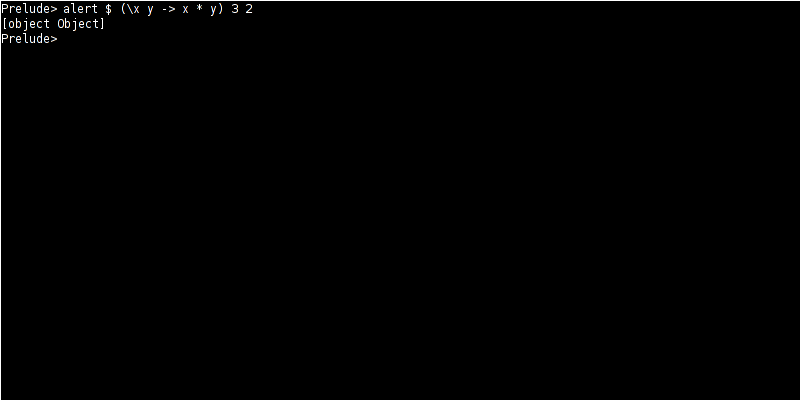
\includegraphics[width=1\textwidth]{hiji_screen3.png}
        \caption{HIJi användargränssnitt}
        \label{fig:hiji} % Labels must come after caption!
    \end{center}
\end{figure}

Figur \ref{fig:hiji} visar hur HIJi ser ut. De första raderna visar, precis som i GHCi, vilka moduler som för närvarande är laddade. I det här exemplet är den förladdade modulen Prelude laddad. Därefter följer en kommandotolk där användaren fritt kan skriva in egna funktioner. I figuren är en lambda-funktion inskriven.

HIJi är skapat för att likna GHCi i så stor utsträckning som möjligt.
Genom att efterlikna GHCi kommer användare känna igen sig när de tar steget från HIJi till GHCi. Det blir för dem ett naturligt steg och kortar inlärningströskeln. Även för haskellprogrammerare som är vana användare av GHCi blir det lättare att använda sig av HIJi, de behöver inte fundera hur verktyget ska användas.
